\subsection{Ampersand core in wet BIG}\label{subsection:ampersand-core-in-wet-big}
With sub-question "\acrlong{RQ2}" we want to know what is in the \acrlong{ca}.
For this appendix~\ref{appendixContentAnalysis} is included.
The \acrlong{ca} contains the Concepts, Relations and Rules (see figure~\ref{fig:LogicalDataModel}).
\begin{figure}[!htp]
    \centering
        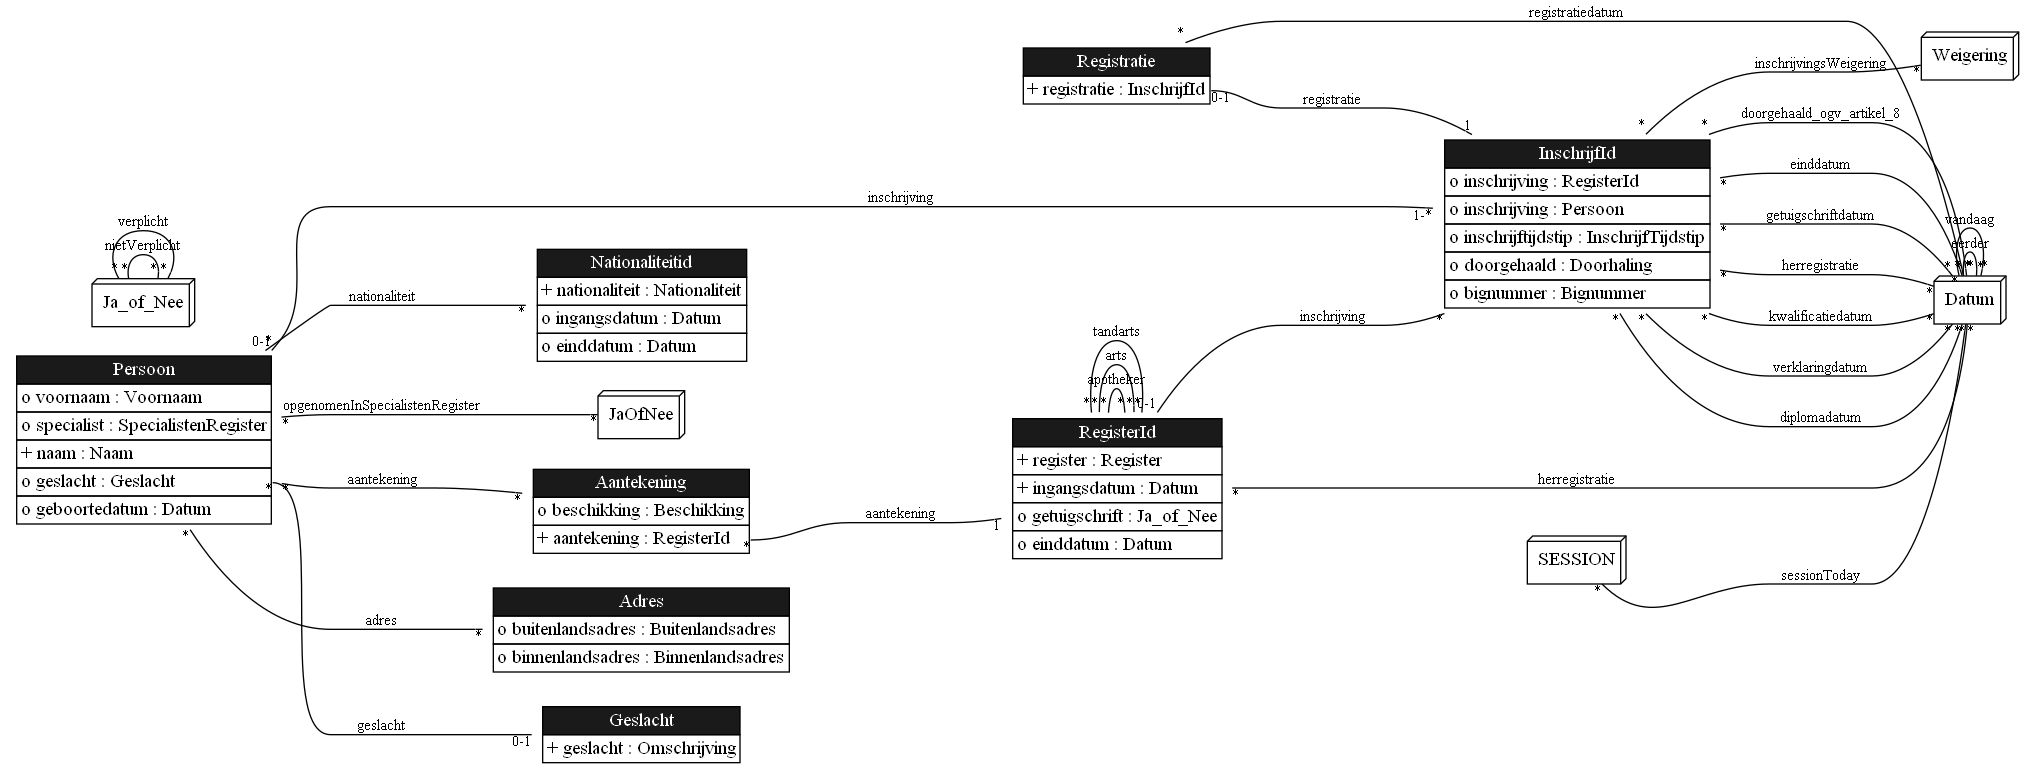
\includegraphics[width=1\textwidth]
            {../images/LogicalDataModel.png}
        \caption{LogicalDataModel from the \acrlong{ca}}
    \label{fig:LogicalDataModel}
\end{figure}
The \acrlong{ca} is not completed because not all articles and related regulations has been analyzed.
The main concepts that appear in the \acrshort{big} are Persoon, Inschrijving, Register, Arts, Tandarts, Apotheker, Gezondheidszorgpsycholoog, Psychotherapeut, Fysiotherapeut, Verloskundige, Verpleegkundige, Physician\_assistant, Orthopedagoog\_generalist, Klinisch\_technoloog, Inschrijfduur, Registratie, Weigering, Aantekening, Geslacht, Nationaliteit, Adres, Specialisme. More Concepts can be identified, but not the entire law and not all associated laws and regulations have been analysed. Not all concepts are interrelated. The Arts and Tandarts do not have a functional relationship, but they do share the relationship to Persoon and Inschrijving.